%% example on how to properly add a picture
% \begin{figure}[h]
%     \centering
%     \includegraphics[width=\linewidth]{example.png}
%     \caption{example}
%     \label{fig:example}
% \end{figure}
End devices in the IoT deployment are often event-driven instead of periodically activated. 
That means that some predefined event has to happen in order to initiate the end device communication with the base station.
Usually, when the end device is mentioned in the context of the IoT, it is expected to have sensors embedded on it and, more importantly, to have connection with some gateway where data is going to be relayed to a network server and, subsequently, to an application server.
When data is collected on the base station it can be formed as:
\begin{description}
    \item[time series data] - a series of data points indexed in time order and taken at successive equally spaced points in time
    \item[sequential non-structured data] - the order of data matters but the period of time between time points is not equal 
\end{description}
Event-driven end devices or, more precisely, end devices that transmit data after they have been triggered by some event captured by the sensor, generate sequential data without any noticable equality in the time period between the two adjacent received data points on the base station end.
If devices are programmed to measure and transmit measured data to the base station, good practice is to keep the transmission equally spaced in time in order to create time series data set.
A time series data is of great interest because it provides possibility of applying forecasting methods by observing possible patterns in historical data. 
Time series forecasting can be termed as the process of predicting the future by understanding the past \cite{Raicharoen_timeseries}.

\section{General overview and main components of time series data}
A time series is a sequential set of data points, measured over successive time and is defined as a set of observations $x(t), t = 0, 1, 2,...$ where $t$ represents the time elapsed and $x(t)$ is treated as a random variable.
If the time series data set is consisted of only single observed variable, it is called univariate and in the case of multiple observed variables, it is termed as a multivariate time series. 
Talking about a standard time series data, there are four important components that affect the shape of a time series data. Those components are: \cite{Adhikari_timeseries}
\begin{itemize}
    \item trend - the tendency of a time series to increase, decrease or stagnate over a long period of time
    \item cyclicality - medium-term changes in a series caused by circumstances, which repeat in cycles
    \item seasonality - variations in a time series characterized by fluctuations within a observed period of time during the season
    \item irregular components - all unpredictable influences which are not regular and are not repeated in a particular pattern; there is no defined statistical technique for measuring a time series with this characteristic (random walks) \cite{timeseries}
\end{itemize}

An important part of the analysis of a time series is the selection of a suitable probability distribution for the data. There is always a strong possibility of future unpredictable behaviour of observed data if each observation $x_{t}$ is a realized value of a certain random variable $X_{t}$.

\section{Time series analysis and forecasting methods}
For statistics, econometrics, quantitative finance, meteorology, and geophysics the primary goal of a time series analysis is forecasting. 
In the context of signal processing, control engineering and communication engineering it is used for a signal detection and estimation.
In the context of data mining, pattern recognition and machine learning a time series analysis can be used for clustering, classification, query by content, anomaly detection as well as forecasting.
Whatever the application of a time series analysis is, it always has to start by reviewing data stationarity, seasonality and possible autocorrelation in the target variable.

The concept of a stationary process in its simplest definition can be defined as a stohastic process with statistical properties such as the mean and the variance independent upon time. 
Stationarity is a necessary condition for building a time series model that is useful for future forecasting. There are two types of stationary processes: 
\begin{itemize}
    \item strict stationary process - a stohastic process whose uncoditional joint probability distribution does not change when shifted in time, consequntly statistical parameters such as the mean and the variance do not change over time
    \item N'th order stationary process - a stohastic process achieved by computing differences between consecutive observations of the same non-strict stationary time series; the method of differencing can help stabilize the mean of time series by removing changes (i.e. trend and seasonality) in the level of the time series
\end{itemize}
In order to identify non-stationarity in the time series, it is important to observe autocorrelation function plot on the target variable. 
The autocorrelation function reflects how the observations in a time series are related to each other. 
The autocorrelation coeficient is well defined in the following formula:
\begin{equation}
    \rho_{k} = \frac{\gamma_{k}}{\gamma_{0}}
\end{equation}
where $\gamma_{k}$ is the autocovariance at a lag $k$ defined as:
\begin{equation}
    \gamma_{k} = Cov(x_{t}, x_{t+k}) = E[(x_{t} - \mu)(x_{t+k} - \mu)]
\end{equation}
and $\mu$ is the mean of the time series.
The atocovariance at the lag zero $\gamma_{0}$ is the variance of the time series. \cite{Adhikari_timeseries}

Another good condition is the ergodicity. 
Statistical properties of an ergodic process can be deduced from a single, sufficiently long, random sample of a process.
The reasoning is that any collection of random samples from a process must represent the average statistical properties of the entire process.

Before computational analysis of a time series data set, intensive cleansing methods should be performed. 
For standard stohastic forecasting models, a time series has to have stationarity property.
There are two widely used linear times series models: \emph{autoregression} (AR) and \emph{moving average} (MA).
Applying the mentioned two linear models on the data simultaneously, we get \emph{autoregressive moving average} (ARMA) which can be enriched with \emph{differentiation} (I) when the stationarity condition is not satisfied.
There are additional extensions to each of the mentioned models that deal with vector-valued data and are available under the heading of the multivariate time series data. 
Extensions on the AR(I)MA model are ARFIMA (autoregressive fractionally integrated moving average) and SARIMA (seasonal autoregressive integrated moving average).
Additional set of extensions of these models is available for use where the observed time series is driven by some \textit{forcing} time series. 
A distinction from the multivariate time series is that the forcing series may be deterministic, thus called exogenous.

Non-linear time series are characterized by changable variance over time (heteroskedasticity property).
For a time series data with non-linear patterns often used forecasting methods are ARCH (autoregressive conditional heteroskedasticity) and its variations GARCH (generalized ARCH), EGARCH (exponential GARCH), etc.

Applying the ARIMA model means that the time series data has no visible seasonality but is non-stationary.
The seasonal ARIMA (SARIMA) model is used for a seasonal, non-stationary time series. 
In this subsection, the basic ARIMA will be explained and visualized using the air passengers data set from \cite{timeseriespython}.
The air passengers data set is consisted of the number of airplane passengers for each month in ten-year period of time and is depicted in fig. \ref{fig:airpassengers}.
\begin{figure}[h]
    \centering
    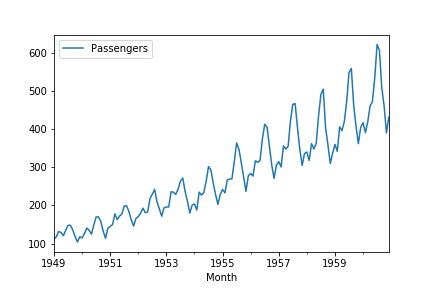
\includegraphics[width=0.7\linewidth]{airpassengers.png}
    \caption{The visualization of the exemplatory time series data: the number of passengers for each month in ten-year time period. This data is obtained from teh Github repository \cite{timeseriespython} which was used at PyCon 2017 talk on a time series analysis}
    \label{fig:airpassengers}
\end{figure}

An ARMA(p, q) model is a combination of AR(p) and MA(q) models. An AR(p) is mathematically defined as:
\begin{equation}
    y_{t} = \beta_{0} + \beta_{1}y_{t-1} + \beta_{2}y_{t-2} + ... + \beta_{n}y_{t-p} = \beta_{0} + \sum_{i=1}^{p}\beta_{i} y_{t-i}
\end{equation}
where the regression happens with past values. $\beta_{i}$ is the model parameter for value in $t-i$ moment. 
Constant $p$ represents the order of the model.

A moving average MA(q) model uses past errors as explanatory variables instead of past values of the series. The mathematical model of a moving average function is defined as:
\begin{equation}
    y_{t} = \mu + \epsilon_{t} + \sigma_{1}\epsilon_{t-1} + \sigma_{2}\epsilon_{t-2} + ... + \sigma_{n}\epsilon_{t-q} = \mu + \epsilon_{t} + \sum_{i=1}^{q}{\sigma_{i} \epsilon_{t-i}}
\end{equation}
where $\mu$ is the mean of the series, $\sigma_{i}$ is the model parameter for the $t-i$ past value moment.
The errors, $\epsilon_{i}$ where $i \in {1, 2, 3, ..., q}$ are considered as explanatory variables and $q$ is the order of the function.
A moving average model is commonly performed for curve smoothing. 

An ARMA model effectively combines an AR and a MA model and creates a general and usefull class of time series models.
Mathematically, an ARMA(p, q) is represented as:
\begin{equation}
    y_{t} = (\beta_{0} + \mu) + \epsilon_{t} + \sum_{i=1}^{p}\beta_{i} y_{t-i} +  \sum_{i=1}^{q}{\sigma_{i} \epsilon_{t-i}}
\end{equation}

Additionally, if the non-stationarity has been confirmed using the autocorrelation and/or the partial autocorrelation function (PACF), differencing should be introduced. 
The additional parameter $d$ controls the level of differencing.
In the case of the air passengers data, fig. \ref{fig:airpassengers}, differencing by $d = 1$ is depicted in fig. \ref{fig:dif}.
\begin{figure}[h]
    \centering
    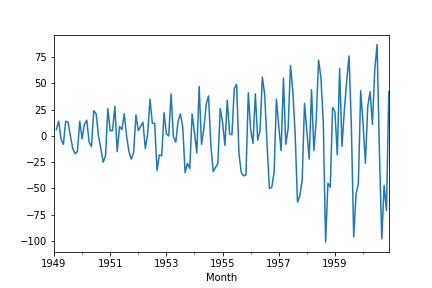
\includegraphics[width=0.7\linewidth]{dif.png}
    \caption{The order 1 differencing function performed on the air passengers data set}
    \label{fig:dif}
\end{figure}
Simple ARIMA model performed on the air passengers data is shown in fig. \ref{fig:arima}. ARIMA parameters p, d and q are configured as 2, 1, 2 respectively. 
\begin{figure}[h]
    \centering
    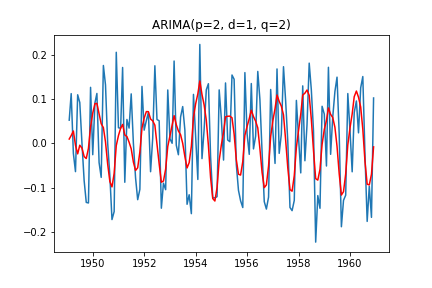
\includegraphics[width=0.7\linewidth]{arima.png}
    \caption{The ARIMA model with parameters p=2, d=1 and q=2 performed on the air passengers data set}
    \label{fig:arima}
\end{figure}

It is fairly obvious that applying described ARIMA model on observed data set is far from perfect but has potential to become strong forecasting method for the time series data when applied correctly.

\section{Introducing artificial neural networks}
Artificial neural networks (ANN) approach for time series modeling and forecasting has reached a great level of importance in the last couple of years.
ANNs are so widely used because of the powerful pattern classification and the pattern recognition cappabilities. 
Since 1940s, ANNs are developed to mimic the intelligence and the mechanism of human brain \cite{ann_history}.
Over the years ANNs have spread out to variaty of different fields such as business, industry and engineering, science, etc. because of the ability to learn from the past experience and provide inference to the output.

\subsection{The ANN architecture and common applications}
The most widely used ANNs in forecasting problems are visualized in fig. \ref{fig:ann}. 
The model has 3 layers: \emph{input layer}, \emph{hidden layer(s)} and \emph{output layer}.
The output of the model is computed using the mathematical expression: \cite{zhang_ann_ts}
\begin{equation}
    y_{t} = \alpha_{0} + \sum_{j=1}^{q}{\alpha_{j}q(\beta_{0j} + \sum_{i=1}^{p}{\beta_{ij}y_{t-1}}) + \epsilon_{t}}
\end{equation}
where $\alpha_{j}$ and $\beta_{ij}$ are the model parameters, $p$ is the number of input nodes and $q$ is the number of hidden nodes, $g$ is the transfer function at the hidden layer, $\epsilon_{t}$ is the random error and, lastly, $\alpha_{0}$ and $\beta_{0j}$ are the bias terms.
The transfer function of the hidden layer(s) for the time series data is a logistic sigmoid function, where $g(x)$ is applied as the nonlinear activation function:
\begin{equation}
    g(x) = \frac{1}{1 + \exp^{-x}}
\end{equation}
\begin{figure}[h]
    \centering
    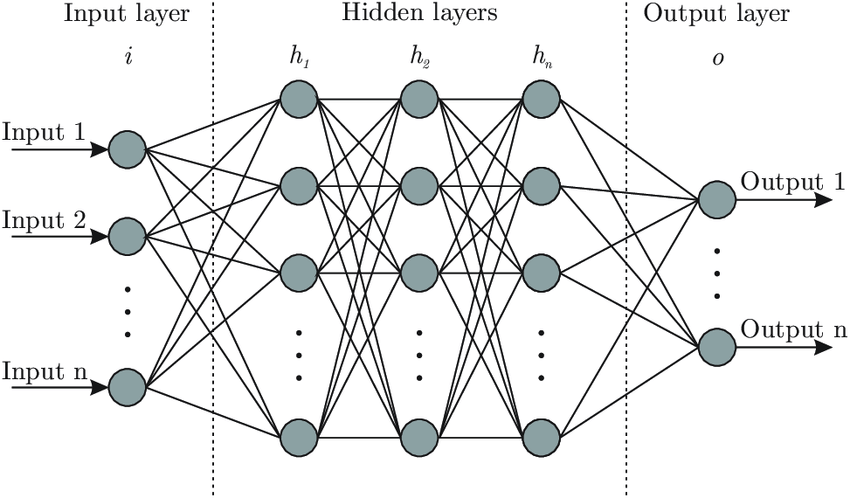
\includegraphics[width=0.8\linewidth]{ann.png}
    \caption{Common visualization of the multi-layer perceptron (MLP) neural network, which uses the hidden layer feed forward network (FNN). The figure was acquired from \cite{ann_architecture}}
    \label{fig:ann}
\end{figure}
The feed forward ANN model described above is the oldest form of the ANN where a non-linear functional mapping is performed from the past observations of the time series to the future value, $y_{t} = f(y_{t-1}, y_{t-2}, ..., y_{t-p}, \textbf{w}) + \epsilon_{t}$, where $\textbf{w}$ is a vector of all parameters and $f$ is a function determined by the network structure and connection weights \cite{Adhikari_timeseries}.

\subsection{Recurrent neural networks for the time series data}
ANNs are good predictors for the time series data because of the three main reasons:
\begin{description}
    \item[data-driven and self-adaptiveness] There is no need to make \textit{a priori} assumptions about statistical distribution of the data before feeding the ANN with the data \cite{Adhikari_timeseries}
    \item[non-linearity] ANNs are perfect for modeling data without obvious patterns  \cite{Zhang_ANN}
    \item[universial functional approximators] Any continuous function can be approximated to any accuracy \cite{Hornik_ANN}  
\end{description}

Even though \textit{vanilla} ANNs are very powerful tool to create predictions based on historical events, they do lack persistence. 
Recurrent neural networks (RNN) are solving this issue implementing loops and allowing information to persist, depcited in fig. \ref{fig:rnn}.
\begin{figure}[h]
    \centering
    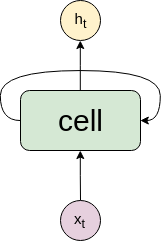
\includegraphics[width=0.2\linewidth]{RNN.png}
    \caption{The recurrent neural network is a version of the artificial neural network with loops in them, allowing the information to persist. The cell looks at the input $x_{t}$ and outputs a value $h_{t}$, while the loop allows the information to be passed from one step of the network to the next \cite{Olah_LSTM}}
    \label{fig:rnn}
\end{figure}

RNNs are using the gradient descent (first-order iterative optimization algorithm, usually used for finding the local minimum of the function) as a way to minimize the error caused by changing each weight in the proportion to the derivative of the error with the respect to that weight.
The main problem with this approach is the error gradient vanishing, which is causing the RNN to become unable to learn how to connect the information if the relevant data is devided by large gap.
The vanishing gradient problem happens when the leading eigenvalue of the weight matrix becomes too small. 
This situation can lead to gradient signal becoming so small that learning becomes extremely slow and, eventually, stops working.
The shrinkage of the gradient during the back propagation is described as:
$$ w_{t} = w_{t-1} - r * gradient $$
where $w_{t}$ and $w_{t-1}$ are weights in the current and the former iteration, and $r$ is learning rate.

The inner workings of the RNN are shown in fig. \ref{fig:rnn-unpacked}.
\begin{figure}[h]
    \centering
    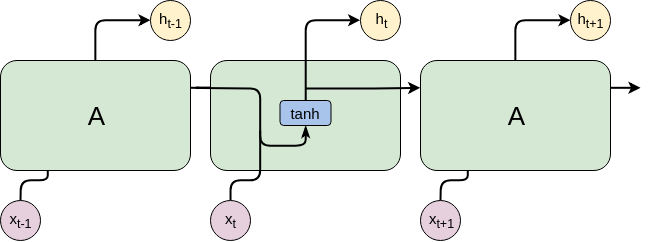
\includegraphics[width=0.8\linewidth]{RNN-unpacked.png}
    \caption{Unpacked recurrent neural network has the form of a chain of repeating cells. Each cell has its own \textit{tanh} activation function}
    \label{fig:rnn-unpacked}
\end{figure}

\subsection{Long short-term memory networks and their improvements for modeling the time series data}
Just like the RNN, long short-term memory (LSTM) network architecture is formed as a chain structure. 
The difference is that every cell has four in-layers, each performing specific operations on the input data and interacting with others in a special way. The general overview of an LSTM network is shown in fig. \ref{fig:lstm}.
\begin{figure}[h]
    \centering
    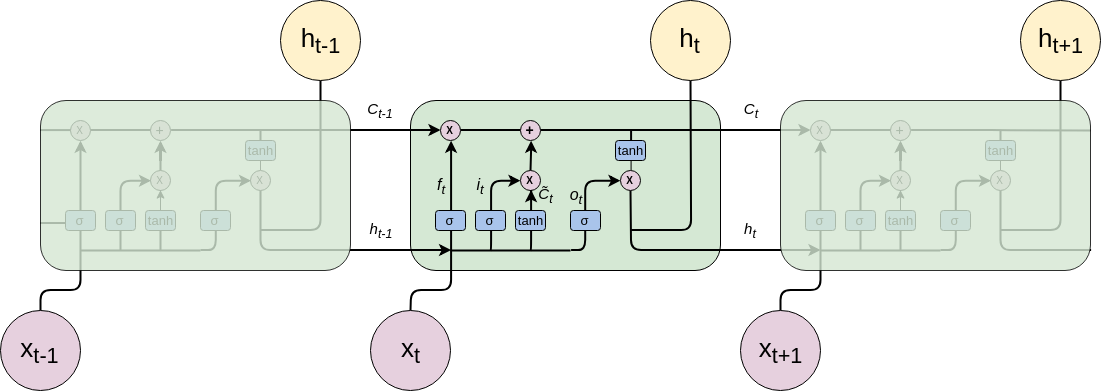
\includegraphics[width=\linewidth]{LSTM.png}
    \caption{LSTM network high-level layout. Each line carries an entire vector - from the output of one node to the input of others. All depicted algebraic operations are pointwise and blue boxes represent different activation function}
    \label{fig:lstm}
\end{figure}
Green boxes represent cells (or neurons) of the network and since the LSTM is recurrant network, both new input $x_{t}$ and the output of the previous cell $h_{t-1}$ are fed to the current cell.

An LSTM cell is consisted of five components which allow it to model both long-term and short-term data: cell state at time $t$ ($C_{t}$), hidden state ($\tilde{C}_{t}$), input gate ($i_{t}$), forget gate ($f_{t}$) and output gate ($o_{t}$).
The cell state, presented with the upper horizontal line in fig. \ref{fig:lstm},  runs through the whole cell and is affected by minor linear changes. 

Inside each LSTM cell, there are mechanisms called \emph{gates} that allow information to be passed in the selective fashion from the LSTM to the cell state. 
There are three types of gates in LSTM network:
\begin{itemize}
	\item {Forget gate} - determines which information to remove from the cell state using \textit{sigmoid} function that outputs value between 0 (completely reject) and 1 (completely accept)
		$$ f_{t} = \sigma (W_{f} \cdot [h_{t-1}, x_{t}] + b_{f}) $$
		where
		\begin{itemize}
			\item[] $ x_{t} $ is the current input vector,
			\item[] $ h_{t-1} $ is the previous cell's output value,
			\item[] $ W_{f} $ is the associated weight,
			\item[] $ b_{f} $ is the added bias.
		\end{itemize}
	\item {Input gate} - decides what new information should be written to the cell state. 
	
	Firstly, the \textit{sigmoid} function decides which value to update:
	$$ i_{t} = \sigma (W_{i} \cdot [h_{t-1}, x_{t}] + b_{i}) $$ 
	where
	\begin{itemize}
		\item[] $ x_{t} $ is the current input vector,
		\item[] $ h_{t-1} $ is the previous cell's output value,
		\item[] $ W_{i} $ is the associated weight,
		\item[] $ b_{i} $ is the added bias.
	\end{itemize}

	After that, the \emph{tanh} layer creates a vector of candidates to be added to the cell state. 
	$$ \tilde{C}_{t} = tanh (W_{C} \cdot [h_{t-1}, x_{t}] + b_{C}) $$
	where
	\begin{itemize}
		\item[] $ x_{t} $ is the current input vector,
		\item[] $ h_{t-1} $ is the previous cell's output value,
		\item[] $ W_{C} $ is the associated weight,
		\item[] $ b_{C} $ is the added bias.
	\end{itemize}
	\item {Output gate} - decides what is going to be the output of the concrete cell. 
	$$ o_{t} = \theta (W_{o} [h_{t-1}, x_{t}] + b_{o}) $$ 
	where
	\begin{itemize}
		\item[] $ x_{t} $ is the current input vector,
		\item[] $ h_{t-1} $ is the previous cell's output value,
		\item[] $ W_{o} $ is the associated weight,
		\item[] $ b_{o} $ is the added bias.
	\end{itemize}
	
	The output is based on the filtered version of the cell state.
	$$ h_{t} = o_{t} \times tanh(C_{t})$$
	where 
	$ C_{t} $ is the new cell state calclulated as:
	$ C_{t} = f_{t} \times C_{t-1} + i_{t} \times \tilde{C}_{t} $
\end{itemize}

An LSTM network is a huge step up considering a RNN. 
The LSTM architecture is proposed in 1997 in \cite{Hochreiter_LSTM} and it found its application in many fields that deal with sequenced data forms.
For this thesis, a LSTM is of the special interest because it is a good fit for a time series data. 

